\chapter{METODOLOGI}
\label{chap:metodologi}

\section{Metode yang dirancang}
\label{sec:metode yang dirancang}

Metode yang dirancang pada penelitian ini sebagaimana ditunjukkan pada Gambar \ref{fig:metode}

\begin{figure}[H]
  \centering
  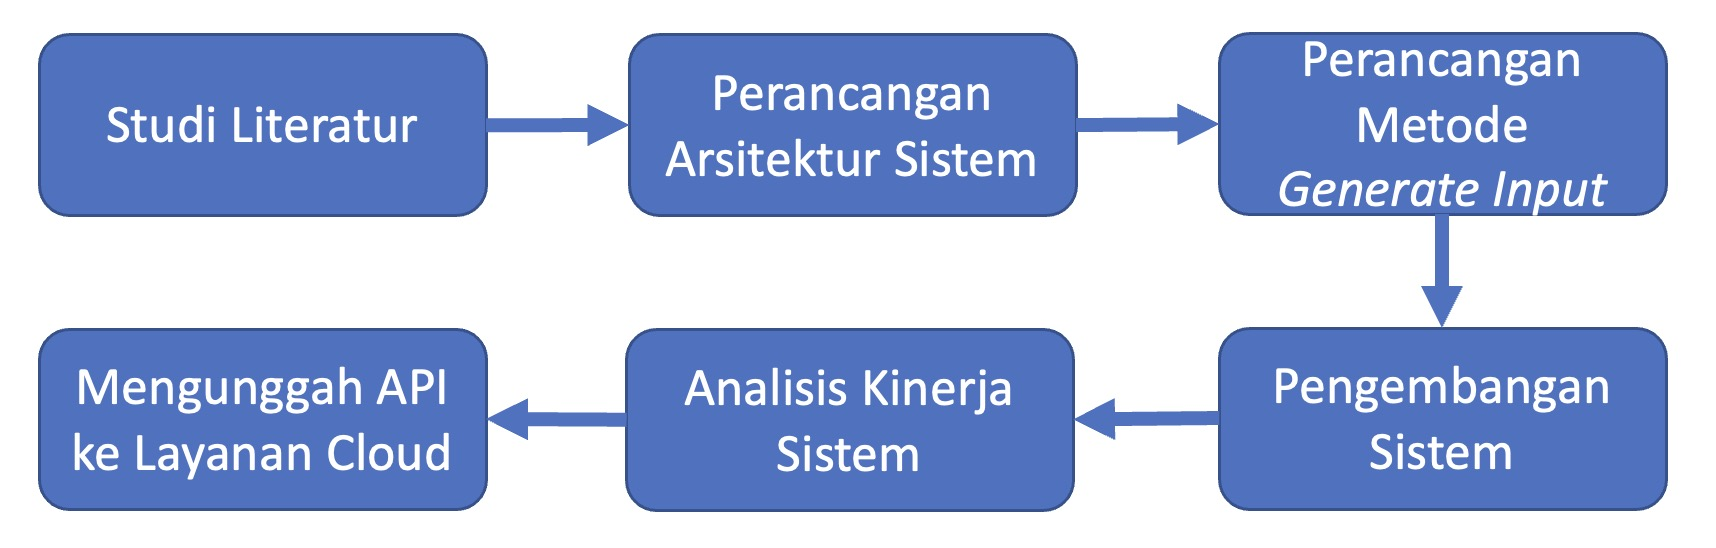
\includegraphics[scale=0.25]{gambar/DiagramAlirMetodePenelitian.jpg}

  % Ubah dengan keterangan gambar yang diinginkan
  \caption{Diagram Alir Metode Penelitian}
  \label{fig:metode}
\end{figure}
% what else except nolistsep?

\begin{itemize}[topsep=0pt]
  \item \textbf{Studi Literatur}
  
  Pada tahap ini dilakukan riset studi literatur mengenai konsep 
  dan permasalahan - permasalahan yang sudah ada terkait DISC, 
  Apache Spark, Titian, DistilGPT2, dan FastAPI. Studi literatur didapatkan melalui buku, internet, jurnal penelitian, dan materi-materi kuliah yang berkaitan dengan metode yang akan digunakan.

  \item \textbf{Perancangan Arsitektur Sistem}
  
  Tahap perancangan arsitektur sistem pada penelitian ini 
  dilakukan dengan mengombinasikan dasar teori dan penelitian 
  terkait pada Bab \ref{chap:tinjauanpustaka}. 
  Perancangan metode akan dimulai dari proses \emph{pre-training}
  terhadap model DistilGPT2 menggunakan baris dataset random dari 
  dataset masing-masing \emph{benchmark program} yang akan 
  diuji. Kemudian program tersebut akan diberikan parameter tertentu 
  agar dapat menghasilkan output yang bermasalah. Setelah itu,
  dengan menggunakan Titian, akan dilakukan proses \emph{provenance data}
  untuk mendapatkan nilai awal dari baris dataset yang menyebabkan
  keluaran yang mencurigakan tersebut. 
  Setelah itu, dilakukan proses re-training lagi terhadap
  model DistilGPT2 menggunakan baris dataset penyebab kesalahan
  tersebut yang kemudian dilakukan proses \emph{generate input}
  baru yang menginduksi kesalahan pada program tersebut dengan jumlah
  yang seminimal mungkin dapat dianalisis oleh \emph{developer}. 
  Hasil dari proses ini kemudian akan dijalankan kembali menggunakan
  program yang sama untuk melihat apakah program tersebut masih
  menghasilkan keluaran yang bermasalah atau tidak.
  Alur keseluruhan proses tersebut dapat dilihat pada 
  Gambar \ref{fig:arsitektur}.


  \begin{figure}[H]
    \centering
    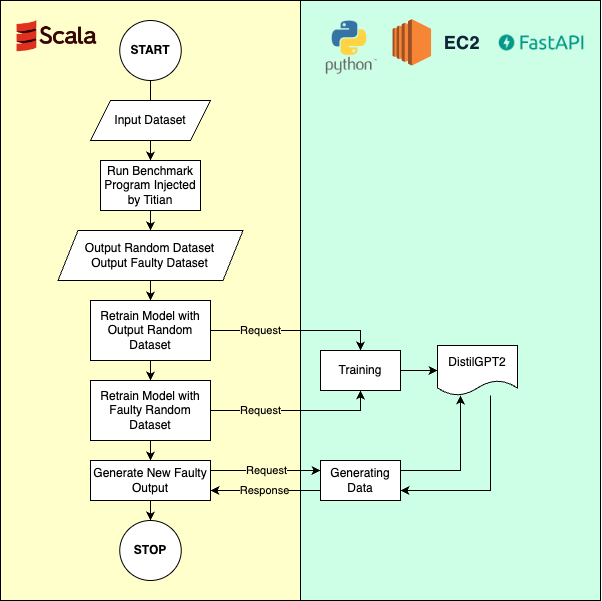
\includegraphics[scale=0.6]{gambar/RancanganArsitekturSistem.png}
  
    % Ubah dengan keterangan gambar yang diinginkan
    \caption{Rancangan Arsitektur Sistem}
    \label{fig:arsitektur}
  \end{figure}

  \item \textbf{Perancangan Metode Generate Input}
  
% endpoint API with FastAPI
% list-model
% - return current, name list

% use-model
% - change current
% —if(not in list)
% 	- make new from base
% - return status

% retrain
% - retrain the model
% - return status

% generate
% - return generate

% reset
% - reset the current from base
% - return status

% delete
% - delete folder current
% - return status

  
  Tahap perancangan metode generate input dilakukan dengan 
  melakukan proses traning dan re-training terhadap 
  DistilGPT2 model yang memiliki \emph{hyperparameter} seperti
  pada Tabel \ref{tab:hyperparameter}.
  Proses ini dilakukan dengan membuat sebuah
  API dengan menggunakan FastAPI yang dapat diakses oleh pengguna. 
  API ini akan memiliki beberapa endpoint yang dapat digunakan 
  oleh pengguna untuk melakukan proses \emph{generate input} baru, 
  \emph{re-training new model}, dan \emph{reset model}. Proses 
  penggunaan API ini dilakukan dalam dua tahap, yaitu \emph{local} 
  dan \emph{cloud} milik Amazon Web Service (AWS).
  Tahap ini dapat ditunjukkan melalui Gambar \ref{fig:generateinput}.

  
  \begin{table}[H]
    \centering
    \caption{Tabel \emph{hyperparameter} model DistilGPT2}
    \begin{tabular}{|p{0.25\linewidth}|p{0.25\linewidth}|}
      \hline
      \textbf{Hyperparameter} & \textbf{Nilai} \\
      \hline
      \raggedright \texttt{learning\_rate} & 5e-4 \\
      \hline
      \raggedright \texttt{warmup\_steps} & 1e2 \\
      \hline
      \raggedright \texttt{epsilon} & 1e-8 \\
      \hline
      \raggedright \texttt{batch\_size} & 2 \\
      \hline
      \raggedright \texttt{epochs} & 10 \\
      \hline
    \end{tabular}
    
    \label{tab:hyperparameter}
  \end{table}


  \begin{figure}[H]
    \centering
    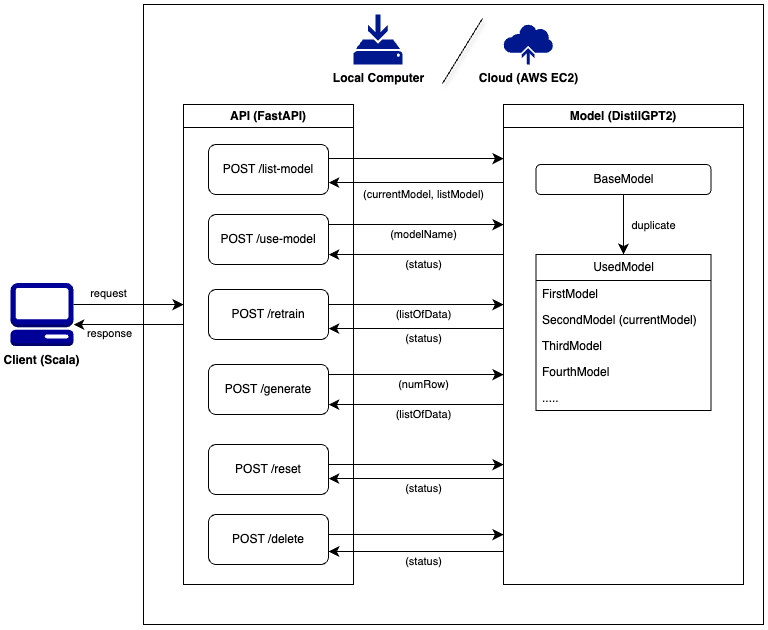
\includegraphics[scale=0.5]{gambar/RancanganMetodeGenerateInput.png}
  
    % Ubah dengan keterangan gambar yang diinginkan
    \caption{Rancangan Metode Generate Input}
    \label{fig:generateinput}

  \end{figure}
  
  \item \textbf{Pengembangan Sistem}\\
  Pengembangan sistem dilakukan dengan menerapkan algoritma
  solusi yang dirancang pada subbab perancangan arsitektur
  sistem dan perancangan metode generate input. Untuk API
  yang dihasilkan pada perancangan metode generate input
  akan menggunakan bahasa pemrograman python, sedangkan
  untuk sistem secara keseluruhan akan menggunakan bahasa
  pemrograman Scala. Untuk masing-masing \emph{benchmark program}
  yang parameter programnya sudah diatur dan telah ditanamkan
  \emph{provenance engine} Titian, akan membuat model baru 
  pada server menggunakan FastAPI berdasarkan \emph{Base Model} 
  yang disediakan. Setelah itu, program tersebut akan melakukan 
  proses \emph{re-training} dan \emph{generate input} baru melalui 
  API tersebut.

  \item \textbf{Analisis Kinerja Sistem}\\
  Analisis kinerja sistem yang akan dilakukan pada penelitian 
  ini ada dua, yaitu tingkat akurasi dan waktu yang dibutuhkan. 
  Terdapat dua poin yang akan diuji pada bagian akurasi yaitu 
  dilakukan dengan membandingkan hasil dari dataset yang tetap 
  mempertahankan kesalahan atau tidak, dan berapa persentase
  jumlah dataset yang berhasil digenerate oleh model untuk
  mereproduksi kesalahan tersebut. Sedangkan pada bagian waktu
  yang dibutuhkan, dilakukan dengan menghitung waktu yang
  dibutuhkan untuk menghasilkan sejumlah dataset yang bermasalah 
  tersebut, dan berapa persentase waktu yang dibutuhkan untuk
  melakukan \emph{re-training} model pada dataset tersebut.

  \item \textbf{Mengunggah API ke Layanan \emph{Cloud}}\\
  Setelah model telah berhasil dilatih untuk menghasilkan 
  input yang menginduksi kesalahan dan diuji untuk memastikan 
  efektivitasnya, langkah selanjutnya adalah mengunggah 
  \emph{API} ke layanan \emph{cloud}. Mengunggah \emph{API} 
  ke layanan \emph{cloud} memungkinkan akses yang mudah dan 
  skalabilitas untuk pengguna di berbagai lokasi. Dengan 
  menggunakan \emph{API} yang diunggah ke \emph{cloud}, 
  pengembang dapat mengotomatisasi proses deteksi dan 
  reproduksi kesalahan tanpa perlu mengelola infrastruktur 
  secara langsung. Layanan \emph{cloud} juga menyediakan 
  sumber daya yang diperlukan untuk menangani permintaan 
  \emph{API} dalam jumlah besar, memastikan bahwa alat 
  tetap responsif dan efisien bahkan di bawah beban kerja 
  yang tinggi. Langkah ini melibatkan konfigurasi server 
  \emph{cloud} untuk menjalankan \emph{LLM} dan mengatur 
  \emph{endpoint API} untuk menerima dan memproses permintaan 
  dari pengguna, memungkinkan integrasi yang mulus dengan 
  berbagai sistem dan aplikasi.

\end{itemize}

\section{Peralatan Pendukung}
\label{sec:peralatan pendukung}

Terdapat beberapa peralatan hardware dan software pendukung yang digunakan untuk pengembangan sistem pada Tugas Akhir ini yang dapat dilihat sebagai berikut:
\begin{itemize}[topsep=0pt]
  \item Hardware
  \begin{enumerate}[topsep=0pt]
    \item Laptop MacBook Pro M2 2022
    \begin{enumerate}[topsep=0pt]
      \item Prosesor: Apple M2
      \item RAM: 8 GB
      \item Storage: 512 GB
      \item GPU: Apple M2
      \item OS: macOS Sonoma
    \end{enumerate}
  \end{enumerate}
  \item Software
  \begin{enumerate}[topsep=0pt]
    \item Google Colaboratory\\
    Digunakan untuk melakukan pelatihan model \emph{DistilGPT2}
    \item Visual Studio Code\\
    Digunakan untuk melakukan pengembangan program FastAPI
    \item IntelliJ IDEA CE\\
    Digunakan untuk melakukan pengembangan program Scala
    \item HuggingFace\\
    Digunakan untuk mengakses model \emph{DistilGPT2}
    \item Amazon Web Service EC2\\
    Digunakan untuk melakukan \emph{deployment} 
    API ke \emph{cloud}
  \end{enumerate}
  \item Sumber Dana
  \begin{enumerate}[topsep=0pt]
    \item LPDP\\  
    Pendaan berasal dari Direktorat Jenderal Pendidikan Tinggi,
    Kementerian Pendidikan, Kebudayaan, Riset, dan Teknologi
    melalui beasiswa \emph{research} Garuda ACE
  \end{enumerate}
\end{itemize}
\section{Implementasi}
\label{sec:implementasi}
Tujuan utama dari penelitian ini adalah menghasilkan data 
yang menyebabkan kesalahan dalam jumlah yang dapat dengan 
mudah dianalisis oleh developer. 
Gambar \ref{fig:alur kerja teknik} merangkum alur 
kerja teknik kami. Teknik ini dimulai 
dengan penyesuaian awal arsitektur \emph{generative LLM} yang 
sudah dilatih sebelumnya menggunakan sampel acak dari data. 
LLM ini di-host di server langsung dan diakses melalui API 
khusus yang dijelaskan pada Tabel \ref{tab:api}.
Ketika ditemukan eksekusi program yang salah, 
penelitian kami menggunakan Titain, sebuah 
\emph{provenance engine}, untuk mendapatkan serangkaian baris yang 
mencurigakan. Sampel data yang dilatih ini  memiliki 
persentase lebih tinggi dari baris yang menyebabkan kesalahan, 
yang kemudian digunakan untuk lebih menyesuaikan generative 
LLM, sehingga model ini mempelajari pola dasar dari input yang 
menyebabkan kesalahan dan cenderung menghasilkan baris 
yang salah. Akhirnya, dengan menggunakan model ini, 
kami mendorongnya untuk menghasilkan 
sampel baris, secara bertahap meningkatkan jumlah baris 
yang dihasilkan hingga \emph{bug} tersebut terdeteksi kembali.
Dalam membuat Tugas Akhir ini, terdapat beberapa proses 
yang perlu dilakukan sesuai pada gambar \ref{fig:diagram alir implementasi}

\begin{figure}[H]
  \centering
  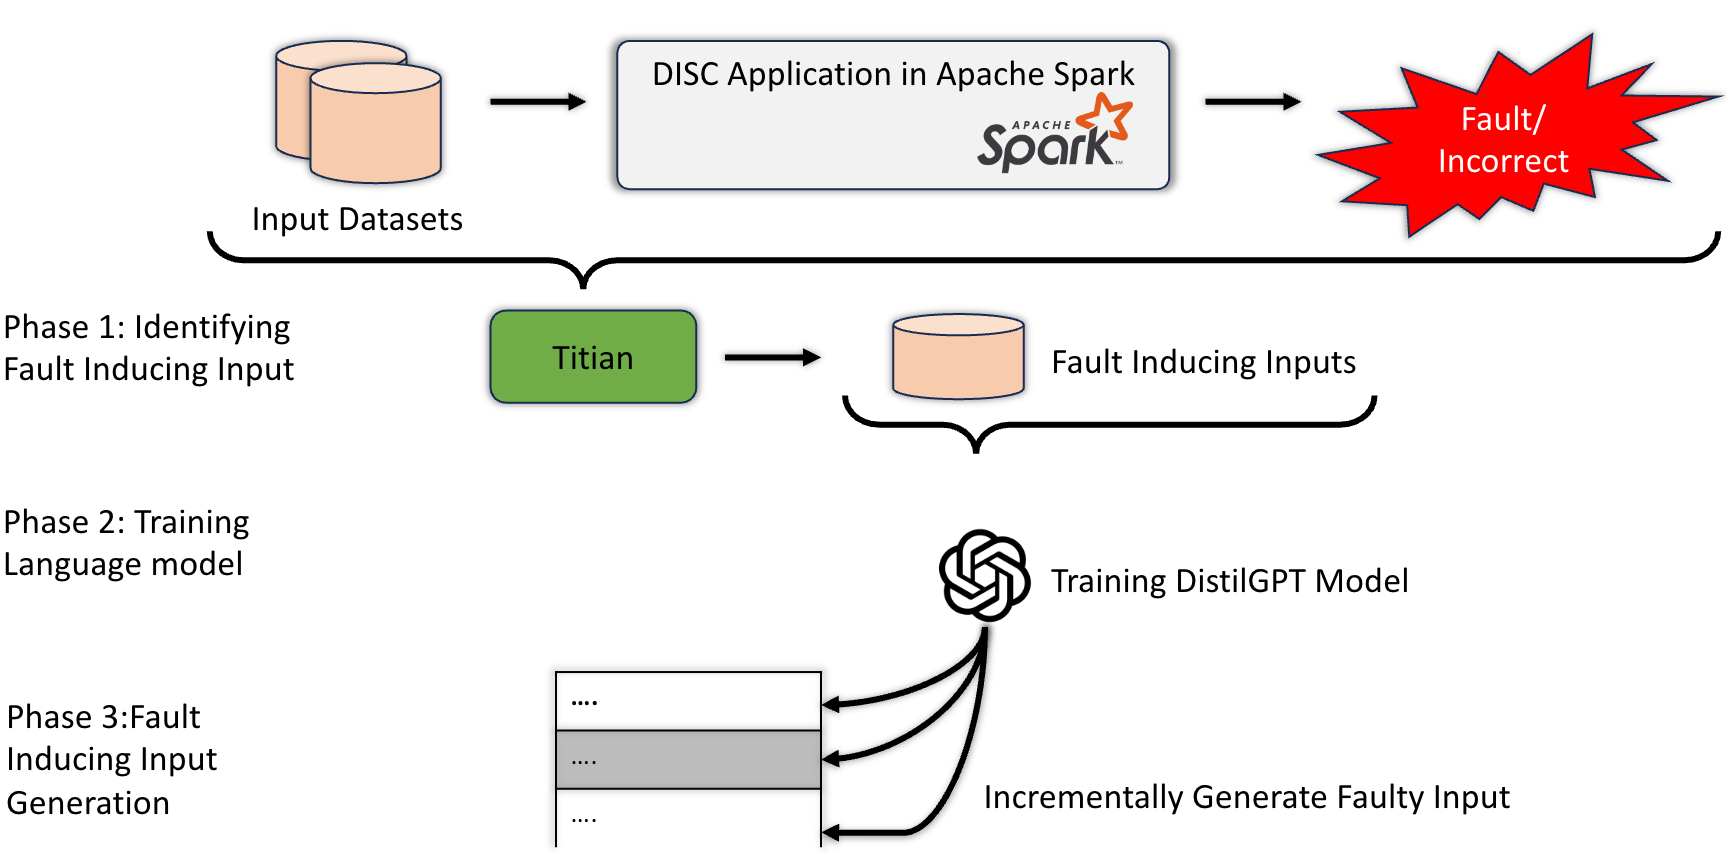
\includegraphics[scale=0.25]{gambar/AlurKerjaTeknik.png}

  % Ubah dengan keterangan gambar yang diinginkan
  \caption{Alur Kerja Teknik}
  \label{fig:alur kerja teknik}
\end{figure}


\begin{table}[H]
  \centering
  \caption{Tabel API}
  \begin{tabular}{|p{0.18\linewidth}|p{0.25\linewidth}|p{0.17\linewidth}|p{0.28\linewidth}|}
    \hline
    \textbf{API} & \textbf{Deskripsi} & \textbf{Request Value}  & \textbf{Response Value} \\
    \hline
    \raggedright \texttt{POST /list-model} &\raggedright Menampilkan model yang terpakai dan tersedia & - &  current\_model, model\_list \\
    \hline
    \raggedright \texttt{POST /use-model} &\raggedright Mengganti model yang terpakai & model\_name & status \\
    \hline
    \texttt{POST /retrain} &\raggedright Melatih ulang model & dataset & status \\
    \hline
    \raggedright \texttt{POST /generate} &\raggedright Menghasilkan input yang menginduksi kesalahan & num\_row & list\_of\_generated\_row \\
    \hline
    \texttt{POST /reset} &\raggedright Mengembalikan model ke model dasar & - & status \\
    \hline
    \texttt{POST /delete} &\raggedright Menghapus model yang terpakai & - & status \\
    \hline
  \end{tabular}
  \label{tab:api}
\end{table}

\begin{figure}[H]
  \centering
  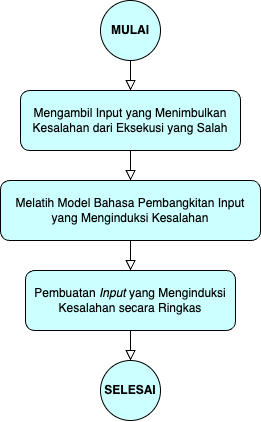
\includegraphics[scale=0.8]{gambar/DiagramAlirRencanaImplementasiDanUjiCoba.png}

  % Ubah dengan keterangan gambar yang diinginkan
  \caption{Diagram Alir Rencana Implementasi dan Uji Coba}
  \label{fig:diagram alir implementasi}
\end{figure}

\subsection{Mengambil Input yang Menimbulkan Kesalahan dari Eksekusi yang Salah}
\label{sec:mengambil input}

Alat kami pertama-tama menggunakan \emph{provenance tool} 
seperti Titian untuk mendapatkan sampel input yang bias 
terhadap baris-baris yang menginduksi kesalahan dalam eksekusi 
program tertentu. Ketika analis data mengeksekusi program 
dengan data asli, alat kami menggunakan \emph{API call} 
{\tt retrain(orig\_dataset)} untuk memberikan data 
awal ke server \emph{LLM}. Tujuan dari data ini adalah untuk 
membiasakan \emph{LLM} dengan format dan skema data. 
Perlu dicatat bahwa karena \emph{LLM} menggunakan 
\emph{pre-trained weights} dari DistilGPT2, tidak diperlukan 
sejumlah besar data untuk dapat menghasilkan baris dengan 
format yang diharapkan. Akibatnya, waktu pelatihan untuk 
langkah ini relatif singkat.

Ketika eksekusi program menghasilkan keluaran yang 
mencurigakan, analis dapat menentukan aturan filter 
menggunakan Titian untuk mengidentifikasi 
kemungkinan penyebab keluaran yang salah. Data penyebab 
yang dikembalikan oleh Titian bisa sangat besar sehingga 
tidak mungkin dianalisis oleh pengembang manusia, misalnya, 
hingga jutaan baris. Wawasan kami adalah bahwa meskipun data 
penyebabnya besar, inti dari kesalahan dapat ditangkap dalam 
beberapa baris saja. Model bahasa modern adalah alat yang 
berguna untuk menangkap pola-pola yang menginduksi kesalahan 
dari sampel bias yang dikembalikan oleh Titian. 
Alur kerja penggunaan Titian pada \emph{benchmark program}
dapat dilihat pada Gambar \ref{fig:diagramofprogramwithtitian}.

\begin{figure}[H]
  \centering
  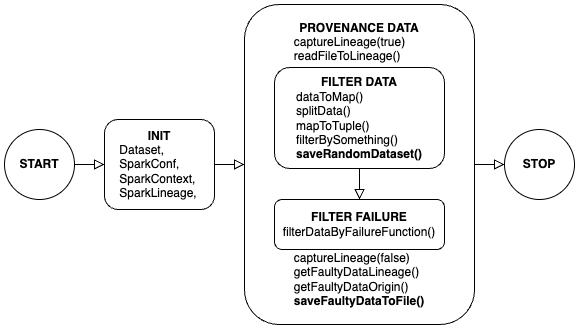
\includegraphics[scale=0.75]{gambar/DiagramOfProgramWithTitian.png}

  % Ubah dengan keterangan gambar yang diinginkan
  \caption{Diagram Alur Kerja Program dengan Titian}
  \label{fig:diagramofprogramwithtitian}
\end{figure}

\subsection{Melatih Model Bahasa Pembangkitan Input yang Menginduksi Kesalahan}
\label{sec:melatih model}

Setelah sekumpulan baris potensial yang menyebabkan keluaran 
yang salah diperoleh, alat kami menggunakan \emph{API call} 
{\tt retrain(faulty\_sample)} untuk melatih ulang model 
dengan data yang dicurigai dan membiasakannya untuk 
menghasilkan input yang menginduksi kesalahan. \emph{LLM} 
mengambil baris-baris ini dan menerapkan proses pelatihan 
awal sekali lagi menggunakan baris-baris yang salah yang 
disediakan. 

% API endpoint
% list-model()
% - return (current_model, model_list)

% use-model(model_name)
% - change current
% —if(not in list)
% 	- make new from base
% - return status

% retrain(all_data)
% - retrain the model
% - return status

% generate(num_row)
% - return list_of_generated_row

% reset()
% - reset the current from base
% - return status

% delete()
% - delete folder current
% - return status

\subsection{Pembuatan \emph{Input} yang Menginduksi Kesalahan secara Ringkas}
\label{sec:pembuatan input}

Dengan menggunakan model yang bias, alat kami dapat 
menghasilkan input baru yang menginduksi kesalahan untuk 
mereproduksi gejala kesalahan yang sama dengan data yang 
jauh lebih sedikit. Karena model yang dilatih adalah 
\emph{generative LLM}, kami dapat menggunakan 
\emph{API call} {\tt generate(N)} untuk menghasilkan 
N baris data. Idealnya, N yang dibutuhkan untuk mereproduksi 
kesalahan harus cukup kecil agar mudah dianalisis oleh 
programmer manusia. Secara analitis, menentukan nilai N 
sangat sulit, jika tidak bisa dibilang mustahil. Oleh 
karena itu, alat kami mengambil pendekatan iteratif. 
Alat ini memulai dengan memanggil {\tt generate(1)} 
dan mengeksekusi program menggunakan baris yang dihasilkan. 
Jika gejala kesalahan terproduksi, \emph{loop} berhenti. Jika tidak, 
alat ini meningkatkan N secara logaritmik hingga kesalahan 
terproduksi. Jika alat ini tidak dapat mereproduksi kesalahan 
dalam jumlah iterasi yang ditentukan oleh pengguna, loop akan 
dihentikan dan alat melaporkan kegagalan untuk mereproduksi 
kesalahan. \emph{Pseudocode} dari algoritma ini dapat dilihat pada kode
\ref{lst:scala-api-pseudocode}.

\lstinputlisting[
  caption={\emph{Pseudocode} penggunaan API pada Scala},
  label={lst:scala-api-pseudocode}
]{program/scala-api-pseudocode.txt}

Untuk dapat lebih memahami tentang \emph{pseudocode} 
\ref{lst:scala-api-pseudocode}, kami akan menjelaskan
beberapa bagian dari \emph{pseudocode} tersebut.
Pada \textbf{baris 1}, sebuah daftar ('list') bernama 
'percentageOutput' didefinisikan dengan nilai-nilai 
persentase yang akan digunakan untuk menentukan ukuran 
dataset baru yang akan dihasilkan. \textbf{Baris 4} mengirimkan 
permintaan untuk menggunakan model tertentu yang terkait 
dengan aplikasi yang ditentukan oleh 'appName'. 
Status dari permintaan ini disimpan dalam variabel 
'useModelStatus'. \textbf{Baris 7} mengirimkan permintaan 
untuk mendapatkan model yang sedang digunakan 
('currentModel') dan daftar model yang tersedia 
('modelList'). \textbf{Baris 9-10} mengecek apakah status 
permintaan untuk menggunakan model adalah "Success". 
Jika tidak, sistem akan dihentikan. \textbf{Baris 12} membaca 
semua data dari file 'all\_data.csv' yang berada di 
\emph{path} tertentu dan menyimpannya dalam variabel 
'allData'. \textbf{Baris 15} memilih data acak dari 'allData', 
menggabungkannya dengan pemisah "\#\#\#", dan mengirim 
permintaan untuk melatih ulang model menggunakan data 
acak tersebut. Status permintaan pelatihan ulang 
disimpan dalam variabel 'retrainStatus'. \textbf{Baris 17} 
membaca data yang salah dari file 'incorrect\_data.csv' 
yang berada di path tertentu dan menyimpannya dalam 
variabel 'faultyData'. \textbf{Baris 20} menggabungkan data 
yang salah dengan pemisah "\#\#\#" dan mengirim 
permintaan untuk melatih ulang model menggunakan 
data yang salah tersebut. Status permintaan 
pelatihan ulang disimpan dalam variabel 'retrainStatus'.
\textbf{Baris 22-23} mengecek apakah status permintaan pelatihan 
ulang adalah "Success". Jika tidak, sistem akan dihentikan.

Pada \textbf{baris 26-29}, untuk setiap persentase dalam 
'percentageOutput', jumlah baris ('numRow') yang 
sesuai dihitung berdasarkan persentase dari panjang 'allData'. 
Kemudian, permintaan untuk menghasilkan input baru 
sebesar 'numRow' dikirimkan dan dataset baru disimpan 
dalam file dengan nama yang sesuai dengan jumlah baris.
\textbf{Baris 32} mengirim permintaan untuk mereset model. 
Status permintaan reset disimpan dalam variabel 
'resetModelStatus' yang kemudian pada \textbf{baris 34-35}
dilakukan pengecekan apakah status permintaan 
reset adalah "Success". Jika tidak, sistem akan dihentikan.
\textbf{Baris 38} mengirim permintaan untuk menghapus model
yang sedang digunakan. Status permintaan hapus
disimpan dalam variabel 'deleteModelStatus' yang
kemudian pada \textbf{baris 40-41} dilakukan pengecekan apakah
status permintaan hapus adalah "Success". Jika tidak,
sistem akan dihentikan. Pada \textbf{baris 43}, sistem akan
dihentikan setelah semua operasi selesai.



